Now, the effect of the constraint length is investigated by fixing the code rate. It has been chosen to fix the code rate at 1/2, and use codes with constraint length $7$, $4$ and $3$, i.e. Code 1, Code 4 and Code 5, as specified in table \ref{tab:codeRate}.
\\[6pt]
Figure \ref{fig:constantCodeRateRandomFigure} indicates that increasing the constraint length reduces the amount of errors in the BSC, as expected. It is noticed that at some point, the CER becomes too great for the constraint length to be of any use, making Code 1 with the highest constraint length perform worse after the CER passes $0.08$.
The effect of burst errors is first examined in figure \ref{fig:constantCodeRateBurstFigure}. The codes seem to perform approximately equally well, but with the higher code rate being a slight advantage. This is also seen in the MBEC, shown on figure \ref{fig:constantCodeRateMarkovFigure}, where the performance is almost similar, but with the higher constraint length codes performing better up to some point, as was also noticed in the BSC.
It can thus be concluded that increasing the constraint length do reduce the BER, unless the CER becomes too big, when the additional memory cannot be utilized properly.

%
%This section presents the results obtained by coding the messages with codes having the same code rate (in our case 1/2) but different constraint lengths. Figure \ref{fig:constantCodeRateRandomFigure} indicates that having a higher constraint length reduced the number of decoded errors. However, this is true only for relatively small channel error rates. It can be seen in figure \ref{fig:constantCodeRateRandomFigure} that for our examples, the code with the highest constraint length starts to perform worse than the other at a channel error rate close to 0.08. 
%The results of the simulation performed using a channel that introduces bursts errors are shown in figures \ref{fig:constantCodeRateBurstFigure} and \ref{fig:constantCodeRateMarkovFigure}. In these figures we can see that all the codes perform similarly under burst error conditions. The only observation is that the codes having a smaller constraint length perform slightly better when the channel error rate is low. This advantage is however, reduced when the error rate increases, as it can be seen on Code 3 in figure \ref{fig:constantCodeRateMarkovFigure}.


\begin{figure}
\centering
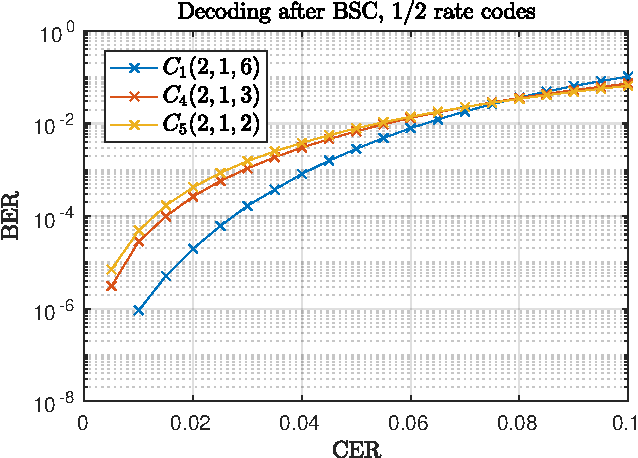
\includegraphics[scale=1]{../figures/extra12rand.pdf} 
\caption{\textit{Comparison of 1/2 rate codes with different constraint length in BSC}\label{fig:constantCodeRateRandomFigure}}
\end{figure}

\begin{figure}
\centering
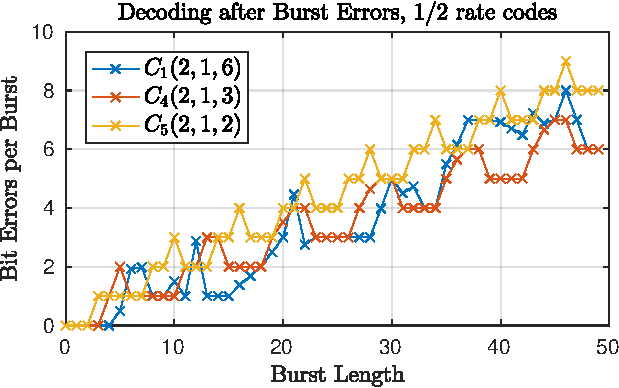
\includegraphics[scale=1]{../figures/extra12burst.pdf} 
\caption{\textit{Comparison of 1/2 rate codes with different constraint length burst correction capabilities}\label{fig:constantCodeRateBurstFigure}}
\end{figure}

\begin{figure}
\centering
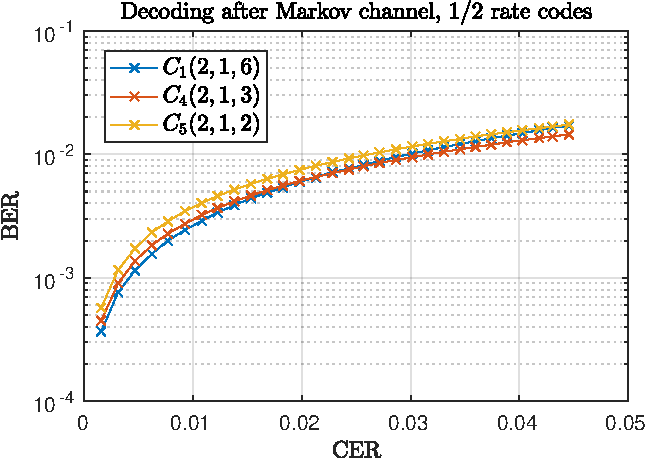
\includegraphics[scale=1]{../figures/extra12markov.pdf} 
\caption{\textit{Comparison of 1/2 rate codes with different constraint length in MBEC}\label{fig:constantCodeRateMarkovFigure}}
\end{figure}
